\usepackage[authoryear,round]{natbib}
\hypersetup{
  colorlinks,
  citecolor=black
}
\newcommand{\sheetnum}{%
	04
}
%\setcounter{section}{\sheetnum-3}
\newcommand{\tutorialtitle}{%
    Gradient methods for parameter optimization
}
\newcommand{\tutorialtitleshort}{%
	Gradient methods
}
% for slides
\subtitle{\sheetnum \tutorialtitle}

\maxdeadcycles=1000 % Workaround for ! Output loop---100 consecutive dead cycles because of too many figures

% The following use of algroithms does not work well with the notes:
%
%
%
%
% instead use the following for your algorithms:
%
%\begin{figure}[!t]
%\removelatexerror
%\begin{algorithm}[H]
    % your algo here
    %\label{alg:algolabel}
    %\caption{algocaption}
%\end{algorithm}
%\end{figure}
%\begin{algorithm}
% Below is the definition for the command \removelatexerror:
\makeatletter
\newcommand{\removelatexerror}{\let\@latex@error\@gobble}
\makeatother

\begin{document} %%%%%%%%%%%%%%%%%%%%%%%%%%%%%%%%%%%%%%%%%%%%%%%%%%%%%%%

\sheet{\sheetnum}{\tutorialtitleshort}

\ttopic{\tutorialtitle}

\columnratio{0.2,0.8}\textbf{}
\begin{paracol}{2}
%\setlength{\columnseprule}{0.1pt}
%\setlength{\columnsep}{5em}

\begin{rightcolumn}

% notes version will ignore it
\begin{frame}
\titlepage
\end{frame}

\begin{frame}
\tableofcontents
\end{frame}


\mode<all>
\section{Linear neuron for regression: analytical solution}

\subsection{Data, Model and Objective}

\begin{frame}\frametitle{Setting}

\underline{Data}:\\

\begin{table}[h]
\begin{tabular}{rl}
obserrvations & $x \in \R$ \\
label         & $y_{T} \in \R$ \\
Dataset       & 
$
\Big\{
	\left(x^{(1)}, y_T^{(1)} 
	\right)
	\,,\, \ldots \,,\,
	\left( x^{(\alpha)}, y_T^{(\alpha)} \right)
	\,,\, \ldots \,,\, 
	\left( x^{(p)}, y_T^{(p)} \right) 
\Big\}
$
\end{tabular}
\end{table}

\pause

\underline{Model}:\\

linear neuron:
\begin{equation}
    y(x; \vec w) = w_{0} + w_{1} x = \vec w^{\top} \vec x
\end{equation}

with $\vec x := (1, x)^{\top} \in \R^{2}$ and $\vec w := (w_{0}, w_{1})^{\top} \in \R^{2}$

\end{frame}

\begin{frame}

\underline{Cost function}:\\

Quadratic error

\begin{align}
E^{T} &= \frac{1}{p} \sum_{\alpha=1}^{p} \;
\frac{1}{2} \, \left( y(x^{(\alpha)}; \vec w)- y^{(\alpha)}_{T}\right)^{2}\\
&= \frac{1}{p} \sum_{\alpha=1}^{p}
\;e^{(\alpha)}
\end{align}

\mode<article>{
The term $\frac{1}{2}$ is merely for convinience when computing the gradient later.
}

\pause

\underline{Optimization}:\\

\begin{align}
E^{T} &\eqexcl \min_{\vec w}\\
\frac{\partial E^{T}}{\partial \vec w} &= \vec 0 \qquad\qquad \text{(satisfied by extrema)}
\label{eq:extremacond}
\end{align}
    
\end{frame}

\newpage

\subsection{Calculating the gradient}

%\mode<article>{
%Finding extrema that satisfy \eqref{eq:extremacond}:
%}

\begin{frame}\frametitle{\subsecname}
 
% temporarily change footnote marks to symbols so not to confuse with exponents
\renewcommand*{\thefootnote}{\fnsymbol{footnote}}    

\begin{align}
\frac{\partial E^{T}}{\partial \vec w} 
\;\;&=\;\; 
\frac{1}{p} \sum_{\alpha=1}^{p} \; 
\frac{\partial e^{(\alpha)}}{\partial \vec w}\\
\;\;&\stackrel{\mathclap{
\substack{\text{chain}\\\text{rule}}}
}
{=}\;\;
\frac{1}{p} \sum_{\alpha=1}^{p} \;
{\color{blue}
\frac{\partial e^{(\alpha)}}{\partial y(x^{(\alpha)};\vec w)}
} 
\cdot
{\color{orange}
\frac{\partial y(x^{(\alpha)};\vec w)}{\partial \vec w}
}\\
\;\;&=\;\;
\frac{1}{p} \sum_{\alpha=1}^{p} \;
{\color{blue}
\big( y(x^{(\alpha)}; \vec w) - y_{T}^{(\alpha)} \big)
}
\cdot
{\color{orange}
\frac{\partial}{\partial \vec w} \vec w^{\top} \vec x^{(\alpha)}
}
%} \;\footnotemark \\
\intertext{using $\frac{\partial}{\partial \vec a}\left(\vec a^{\top} \vec b\right) = \vec b = (b_{1}, b_{2}, \ldots, b_{N})^{\top}$}
\;\;&=\;\;
\frac{1}{p} \sum_{\alpha=1}^{p} \;
{\color{blue}
\big( \vec w^{\top}\vec x^{(\alpha)} - y_{T}^{(\alpha)} \big)
}
\cdot
{\color{orange}
\vec x^{(\alpha)}
}\\
\;\;&=\;\;
\frac{1}{p} \sum_{\alpha=1}^{p} \;
\big( \vec x^{(\alpha)} \, \vec w^{\top}\vec x^{(\alpha)} - \vec x^{(\alpha)} y_{T}^{(\alpha)} \big)\\
%\;\;&=\;\;
%\frac{1}{p} \sum_{\alpha=1}^{p} \;
%{\color{orange}
%\vec x^{(\alpha)}
%}
%\cdot
%{\color{blue}
%\big( {\vec x^{(\alpha)}}^{\top}\vec w - y_{T}^{(\alpha)} \big)
%}\;\footnotemark \\
%\;\;&=\;\;
%\frac{1}{p} \sum_{\alpha=1}^{p} \;
%\Big( 
%{\vec x^{(\alpha)}}^{\top} \kern-.5ex \vec w\; 
%\vec x^{(\alpha)} 
%- y_{T}^{(\alpha)} \vec x^{(\alpha)}
%\Big)\\
\;\;&=:\;\; \vec g
\end{align}    

%\notesonly{ 
%\footnotetext{
%partial derivative calculated by using 
%$y(x^{(\alpha)};\vec w) = \vec w^{\top}\vec x^{(\alpha)}$ and 
%$\frac{\partial}{\partial \vec a}\left(\vec a^{\top} \vec b\right) = \vec b = (b_{1}, b_{2}, \ldots, b_{N})^{\top}$
%}
\footnotetext{
$\vec w^{\top}\vec x^{(\alpha)} = {\vec x^{(\alpha)}}^{\top} \vec w$
}
%}

% change footnote marks back to original scheme (numbers)
\renewcommand*{\thefootnote}{\arabic{footnote}}

\end{frame}

\subsection{Finding minima}

\begin{frame}\frametitle{\subsecname}

Constructing the Hessian matrix $\vec H$ to identify minima among the solutions that satisfy \eqref{eq:extremacond}:
\begin{equation}
\vec{H} \equiv \frac{\partial^2 E^T}{\partial\vec{w}^2} =
\left(\begin{array}{cccc}  
  \frac{\partial^2 E^T}{\partial w_0^2} &
  \frac{\partial^2 E^T}{\partial w_0\partial w_1} & \cdots &
  \frac{\partial^2 E^T}{\partial w_0\partial w_N} \\
  \frac{\partial^2 E^T}{\partial w_1\partial w_0} &
  \frac{\partial^2 E^T}{\partial w_1^2} & \cdots &
  \frac{\partial^2 E^T}{\partial w_1\partial w_N} \\
  \vdots & \vdots & \ddots & \vdots \\
  \frac{\partial^2 E^T}{\partial w_N\partial w_0} &
  \frac{\partial^2 E^T}{\partial w_N\partial w_1} & \cdots &
  \frac{\partial^2 E^T}{\partial w_N^2}
\end{array}\right)
\end{equation}

Let $\vec g$ denote the gradient vector: $\vec g = \frac{\partial E^{T}}{\partial \vec w}$. 
We recognize that the i-th \underline{row} in $\vec H$ resembles $\frac{\partial}{\partial w_i}\vec g^\top$.

Therefore,

\begin{align}
\vec H := \frac{\partial}{\partial \vec w}\vec g^\top
\;\;&=\;\;
\frac{1}{p} \sum_{\alpha=1}^{p} \;
\frac{\partial}{\partial \vec w}
\left(
\frac{e^{(\alpha)}}{y(\vec x^{(\alpha)}; \vec w)}
\cdot
\frac{\partial y(x^{(\alpha)};\vec w)}{\partial \vec w} 
\right)^{\kern-1ex\top}\\
\;\;&=\;\;
\frac{1}{p} \sum_{\alpha=1}^{p} \;
\frac{\partial}{\partial \vec w}
%\Big( 
%\vec x^{(\alpha)}
%\left({\vec x^{(\alpha)}}^{\top}\right) \vec w 
%\;-\; 
%\underbrace{
%\vec x^{(\alpha)}
%y_{T}^{(\alpha)} 
%}_{\text{indep. of }\vec w}
%\Big)\\
\Big( \vec x^{(\alpha)} \, \vec w^{\top}\vec x^{(\alpha)} - \vec x^{(\alpha)} y_{T}^{(\alpha)} \Big)^\top
\intertext{$
{\scriptstyle
\big(\vec x^{(\alpha)} (\vec w^{\top}\vec x^{(\alpha)})\big)^\top 
=~(\vec w^{\top}\vec x^{(\alpha)})^{\top}{\vec x^{(\alpha)}}^{\top}
=~{\vec x^{(\alpha)}}^{\top} \vec w~{\vec x^{(\alpha)}}^{\top}
}
$}
\;\;&=\;\;
\frac{1}{p} \sum_{\alpha=1}^{p} \;
\frac{\partial}{\partial \vec w}
~{\vec x^{(\alpha)}}^{\top} \vec w~{\vec x^{(\alpha)}}^{\top}
-
\frac{\partial}{\partial \vec w}
\underbrace{
\Big(\vec x^{(\alpha)} y_{T}^{(\alpha)} \Big)^\top
}_{\text{indep. of }\vec w}
%\Big( \vec x^{(\alpha)} \, \vec w^{\top}\vec x^{(\alpha)} - \vec x^{(\alpha)}^\top y_{T}^{(\alpha)} \Big)\\
\intertext{
using $\scriptstyle \frac{\partial~\vec a^{\top}\vec B~\vec c}{\partial \vec B} = ~\vec a~\vec b^{\top}$
}
\;\;&=\;\;
\frac{1}{p} \sum_{\alpha=1}^{p} \;
\frac{\partial}{\partial \vec w}
\Big( \vec x^{(\alpha)} \, \vec w^{\top}\vec x^{(\alpha)} - \vec x^{(\alpha)} y_{T}^{(\alpha)} \Big)^\top
\end{align}

\end{frame}

\mode*

\clearpage

\mode<all>
\section{Gradient methods}

\mode<presentation>{
\begin{frame}
	
    \begin{center} \huge
        \secname
    \end{center}
    
    \pause
    \begin{center}
		
\includegraphics[width=0.3\textwidth]{img/meme_analytical}
    \end{center}
	
\end{frame}
}

\subsection{The need for gradient-based optimization}


\begin{frame}


\notesonly{
We have some cost function we want to minimize but solving the problem analytically is not applicable.

}



\question{In what case(s) do we avoid an analytical solution?}

\pause
\begin{itemize}
	\item We cannot fit all the data into memory.
	\item \notesonly{It involves finding an inverse of a matrix, that is not invertible (e.g. linear regression $(\vec X \, \vec X^\top)^{-1}\vec X \, \vec y_{True}^\top$.
	}
    \slidesonly{
    $$
    \vec w^{*} = (\vec X \, \vec X^\top)^{-1}\vec X \, \vec y_{True}^\top
    $$
    \pause
    but $(\vec X \, \vec X^\top)^{-1}$ is not invertible
    }
    \item \notesonly{There is no closed-form solution for the model we're using (e.g. MLP)}
    \slidesonly{no closed-form solution for our model (e.g. MLP with non-linearities)}
	\item Computing the Hessian is too costly. Newton's method also not applicable.\notesonly{\footnote{
	Newton's method finds the root of a function iteratively using the second-order Taylor expansion of the cost function around a point $\vec w_t$. For more details see Haykin Ch. 3.3.
	}}
	\item Non-stationary data. We cannot easily adapt to changes over time.
\end{itemize}

\end{frame}

\mode<article>{

We therefore opt for Gradient-based optimization which is an iterative optimization procedure. 
In the case of a \emph{minimization} problem one can reduce some cost function $E^T_{[\vec w]}$ by taking steps in the direction of steepest \emph{descent}.
For minimizing some cost function $E^T_{[\vec w]}$ w.r.t. to a set of weights $\vec w$, it follows that, if
}
\begin{frame}\frametitle{Alternative: iterative gradient-based optimization}
\begin{equation}
\vec w_{t+1} = \vec w_t - \underbrace{\eta_t \, \frac{\partial E^T}{\partial \vec w} \Bigg|_{\vec w_t}}_{\text{update}~\Delta \vec w}
\end{equation}
\notesonly{
and a small enough }\slidesonly{with }$\eta_t \in \R^+$, then \notesonly{the cost at the next step $t+1$ will become less or remain unchanged. That is} $E^T_{[\vec w_{t+1}]} \le E^T_{[\vec w_{t}]}$.

\mode<article>{
We refer to $\eta_t$ as the learning rate. It allows us to control the size of the step we take in the direction of the gradient.
\emph{Subtracting} the gradient from the current $\vec w_t$ lets us move against the slope in towards some minimum. 
}
\pause
The behavior of gradient descent can be controlled by modulating 
\begin{itemize}
\item The ``scope'' of the gradient. What do we use for deciding on the direction of the update?
\item The learning rate schedule. How big of a step do we take in the direction of the gradient?
\end{itemize}


\end{frame}

\subsection{``Scope'' of the gradient}

\begin{frame}\frametitle{\subsecname}
\mode<article>{
The scope of the gradient method refers to the amount of data used for deciding on the direction of the gradient.
}
\slidesonly{\vspace{-2mm}}
\renewcommand*{\arraystretch}{1.}{
\begin{table}[h]
\begin{tabular}[c]{r|l|l}
\hline
batch      & 
$\displaystyle
\frac{\partial E^{T}}{\partial \vec w} 
\;=\;
\frac{1}{p} \sum_{\alpha=1}^{p} 
\frac{\partial e^{(\alpha)}}{\partial \vec w}
$ &
\pause
\\[10mm]
\hline
mini-batch & \begin{tabular}[c]{@{}c@{}}
$\displaystyle
\frac{\partial E^{T}}{\partial \vec w} 
\;\approx\;
\frac{1}{|\mathcal{M}|} \sum_{\beta \in \mathcal{M}}^{|\mathcal{M}|} 
\frac{\partial e^{(\beta)}}{\partial \vec w}
$\\
$|\mathcal{M}| \ll p$\\
where $\mathcal{M}$ is a set of indices\\
 sampled randomly \\
 from 
 $\{1,\ldots,p\}$
\end{tabular} 
&
\begin{tabular}[c]{@{}l@{}}
noisy \\
estimate of $E^T$, \\
becomes less noisy with \\
larger $|\mathcal{M}|$
\end{tabular} 
\pause
\\[10mm]
\hline
online     &
\begin{tabular}[c]{@{}c@{}}
$\displaystyle
\frac{\partial E^{T}}{\partial \vec w} 
\;\approx\;
\frac{\partial e^{(\beta)}}{\partial \vec w}
$\\
a single random\\ data point $(\vec x^{(\beta)}, \vec y_T^{(\beta)})$
\end{tabular}    &
\begin{tabular}[c]{@{}l@{}}
very noisy \\
estimate of $E^T$
\end{tabular}\\
\end{tabular}
\end{table}
}
\pause
\slidesonly{\vspace{-5mm}}
\question{Which of these can handle non-stationary data?}

\end{frame}

\subsection{Learning rate schedules}

\begin{frame}\frametitle{Robinns \& Munro condition}

\begin{figure}[ht]
     \centering
     \savebox{\imagebox}{
	 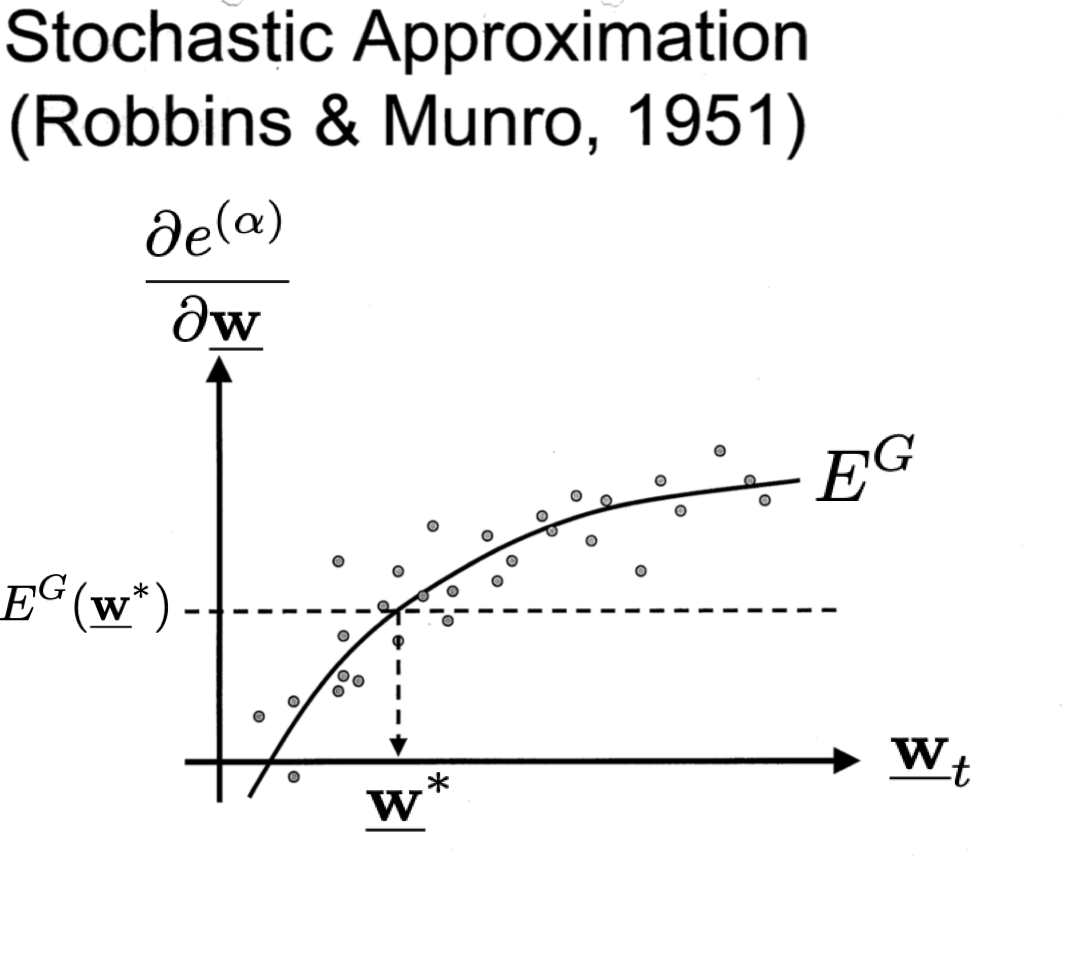
\includegraphics[width=0.5\textwidth]{img/RobbinsMunroNew.png}}%
     \begin{subfigure}[t]{0.35\textwidth}
         \centering
         \usebox{\imagebox}% Place largest image
         \notesonly{\caption{}}
     \end{subfigure}
     \hspace{10mm}
     \begin{subfigure}[t]{0.5\textwidth}
         \centering
         \raisebox{\dimexpr.5\ht\imagebox-.5\height}{% Raise smaller image into place
         \only<2>{
         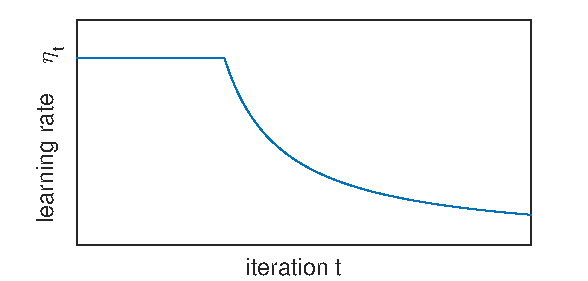
\includegraphics[width=0.99\textwidth]{img/learning_rate-eps-converted-to}
         }
         }
         \notesonly{\caption{}}
     \end{subfigure}
\end{figure}

    
\end{frame}

\begin{frame} \frametitle{Impulse terms}
\mode<article>{
\underline{Impulse terms}:

}
	%\visible<2>{
		\begin{equation*}
			\Delta \vec{w}_{t + 1} \quad=\quad 
			{\color{blue} -{\eta} \frac{\partial E^T}{
				\partial \vec{w}} \bigg|_{\vec{w}_t} } + \;\;
				\underbrace{{\color{red} \mu \; \Delta \vec{w}_t} }_{
					\substack{\text{impulse} \\
						\text{term}}}
		\end{equation*}
	%}
	\vspace{-2cm}
	\only<1>{	
		\begin{center} 
			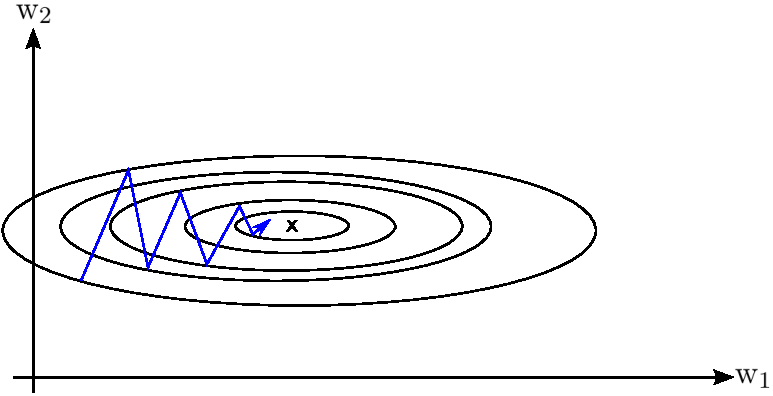
\includegraphics[height=6cm]{img/section1_fig23_clean.pdf} \\
		\end{center}
	} \only<2>{
		\begin{center} 
			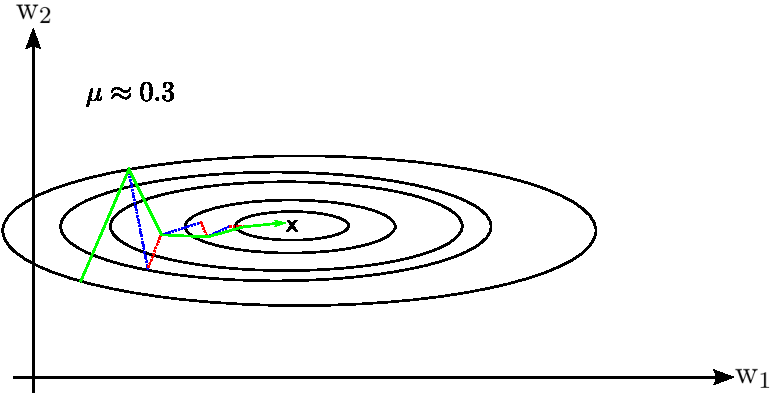
\includegraphics[height=6cm]{img/section1_fig24_clean.pdf}  \\
		\end{center}
	}
\end{frame}

% -----------------------------------------------------------------------------
\begin{frame} \frametitle{Adaptive step size}
 \mode<article>{
\underline{Adaptive step size}:

}   
\begin{center} 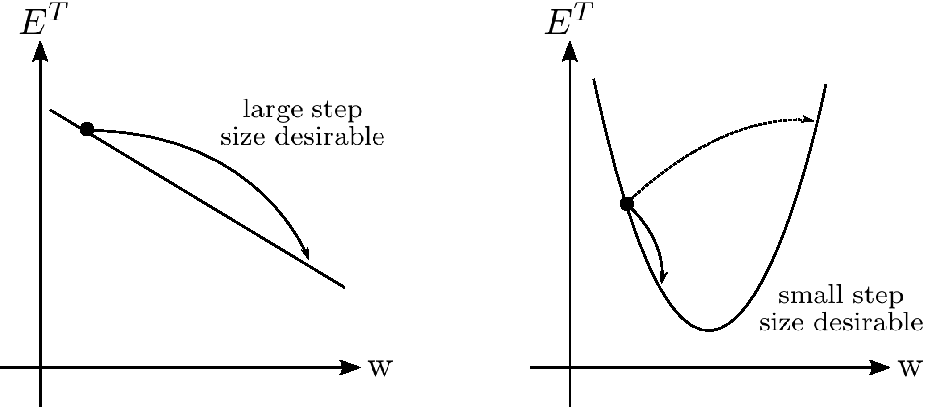
\includegraphics[height=4cm]{img/section1_fig25.pdf} \end{center}
\[ \eta_{t + 1} = \left \{ 
	\begin{array}{lll}
		\rho \eta_t, 
			& \text{if } \Delta E^T < 0,
			& \text{increase step size, if } E^T \downarrow \\
		\delta \eta_t, 
			& \text{if } \Delta E^T > 0,
			& \text{decrease step size, if } E^T \uparrow 
	\end{array} \right.
\]
typical values: $\rho = 1.1, \delta = 0.5$
\end{frame}

% -----------------------------------------------------------------------------
\begin{frame}\frametitle{Line search}
\mode<article>{
\underline{Line search}:

}
   \begin{figure}[h]
    \centering   
    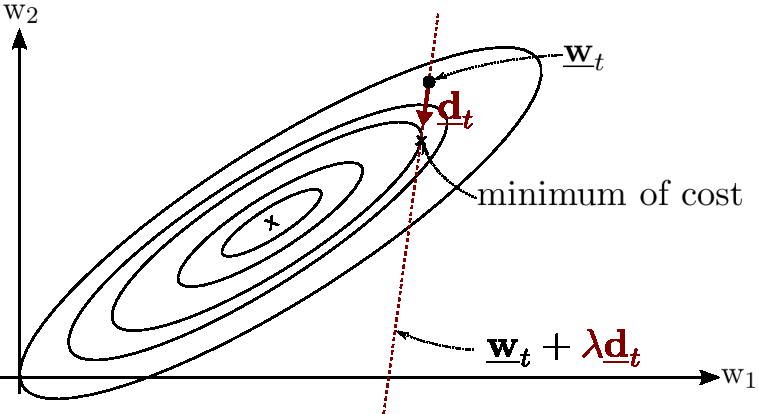
\includegraphics[height=5cm]{img/section1_fig26}
    \mode<article>{
    \caption{Line Search}
    }
    \end{figure}
\end{frame}

\begin{frame}\frametitle{Parabolic interpolation}
\slidesonly{
	\only<1->{\placeimage{9.5}{1}{img/section1_fig26}{width=5cm}}
    \vspace{20mm}
    }
	\begin{center} 
		\includegraphics<1>[height=5cm]{img/parabolicInterpolation_clean_a.pdf} 
		\includegraphics<2>[height=5cm]{img/parabolicInterpolation_clean_b.pdf} 
	\end{center}
\end{frame}


% -----------------------------------------------------------------------------
\begin{frame}\frametitle{Line search}
	\begin{block}{Line search: successive parabolic interpolation}
		\textbf{Initialization:} $a_0, b_0, c_0 \, (\text{on } 
			\vec w_t + \lambda \vec{d}_t);\quad E_{(a_0)}^T,
				\quad E_{(b_0)}^T > E_{(c_0)}^T$
		\vspace{3mm} 

		\While{stopping criterion not fulfilled}{
			\vspace{2mm}
			Fit a parabola through the three points $a_t, b_t, c_t$ \\[2mm]
			Calculate location $d_t$ of its minimum\\[0mm]
			Set $c_{t+1} = d_t,\quad b_{t+1} = c_t,\quad a_{t+1} = \left \{ 
			  \begin{array}{ll}
			 		a_t, & E_{(a_t)}^T < E_{(b_t)}^T \\
			 		b_t, & \text{else}
			 	\end{array} \right.$ 
		}
	\end{block}

	{\scriptsize For details and implementation see 
	e.g.~Numerical Recipes, 2nd edition, Chapter 10.2.}
\end{frame}

\begin{frame}\frametitle{Line search}

\mode<presentation>{
    \begin{center} 
		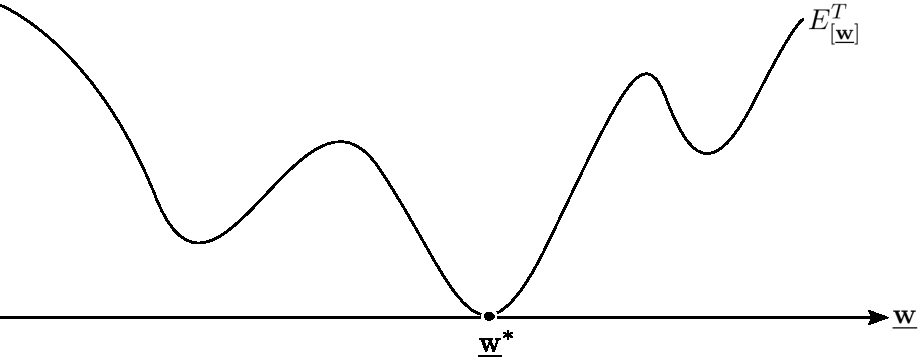
\includegraphics[height=5cm]{img/section1_fig19_no_steps} 
	\end{center}
}

\question{What are potential pitfalls of parabolic interpolation?}

\end{frame}

\begin{frame}\frametitle{Parabolic interpolation}

\mode<presentation>{
    \begin{center}
		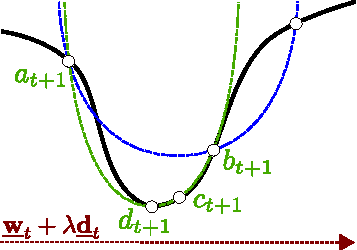
\includegraphics[height=5cm]{img/parabolicInterpolation_clean_b} 
	\end{center}
}

Compute optimal step size:

\begin{equation}
	  \vec{w}_{t+1} = \vec{w}_t - \eta_{t} \vec{g}_t,
	  \qquad \text{with optimal step size} \qquad
	  \eta_{t} = \frac{\vec{g}_t^\top\vec{g}_t}{\vec{g}_t^\top\vec{H}\,\vec{g}_t} \,.
\end{equation}

\end{frame}

\mode*

\clearpage

\mode<all>
\subsection{The Conjugate gradient method}

\subsubsection{Motivation}

\notesonly{
We have seen how line search allows us to reach the minimum along the direction of the gradient $\vec g_t$ computed at time step $t$. It achieves this by manipulating the magnitude of the step we take towards a lower cost.
Looking at what happens over multiple time steps we observe the following movements on the surface of the cost function:
}
\begin{frame}{Limitations of line search}

\begin{center}
	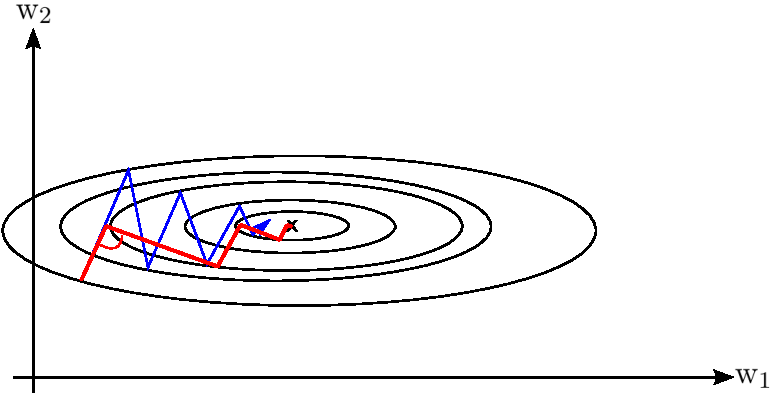
\includegraphics[width=0.6\textwidth]{img/section1_fig23_clean_ls}
	\captionof{figure}{Weight updates by following line search 
	%(\textcolor{red}{red}).}
	(red).}
\end{center}

\mode<presentation>{
	\only<2>{
		\begin{center}
			
\includegraphics[width=0.3\textwidth]{img/meme_point}
		\end{center}
	}
	\only<3>{
		\begin{center}
			
\includegraphics[width=0.3\textwidth]{img/meme_deeper}
		\end{center}
	}
	\only<4>{
		\begin{center}
			
\includegraphics[width=0.3\textwidth]{img/meme_direction}
		\end{center}
	}
}

\end{frame}

\begin{frame}{Limitations of line search}
		\begin{center}
			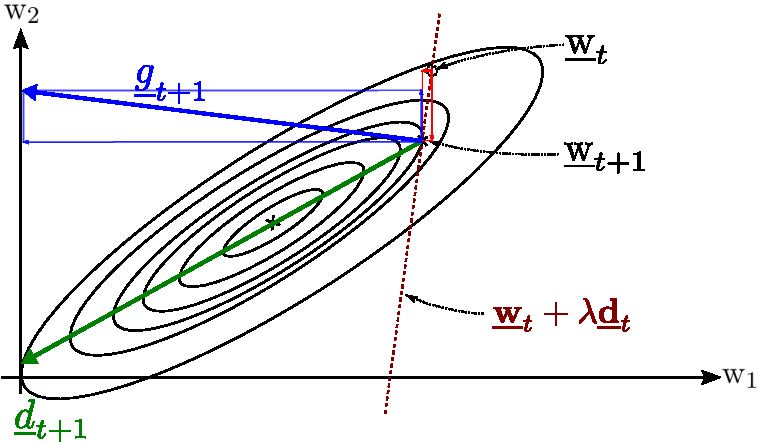
\includegraphics[width=0.8\textwidth]{img/conjugate_direction_c}
			\notesonly{
			\captionof{figure}{The conjugate direction avoids undoing progress made in the previous step.}
			}
		\end{center}
\end{frame}

\begin{frame}\frametitle{Conjugate gradient method}
\mode<article>{
\underline{Conjugate gradient method}:

}

		\begin{eqnarray}
			\vec{w}_{t+1}
			%& = & \mathrm{w}_{ij}(t) 
			%+ \Delta \mathrm{w}_{ij}(t)  \\ 
			& =&  \vec{w}_t + \eta_t \, \vec{d}_{t-1}
		\end{eqnarray}

Don't undo progress of previous search directions $\vec d_{t}$, $\vec d_{t-1}$.

In other words:

The component of the gradient parallel to the old direction $\vec d_{t}$ should
remain zero along the new direction $\vec d_{t+1}$

\pause
	
	\begin{block}{$ $}
		\textbf{Initialization:} $\vec{w},\quad \vec{d} = - \vec{g}$\\
		\vspace{3mm}

		\While{stopping criterion not fulfilled}{
			\vspace{1mm}
			Minimize $E^T$ along $\vec{d}$ using line-search 
				\quad $\rightarrow$ new $\vec{w}$ \\[1mm]
			Calculate the new conjugate direction 
				\quad $\;\,\rightarrow$ new $\vec{d}$
			\vspace{1mm}
		}
	\end{block}

\end{frame}

% -----------------------------------------------------------------------------
\begin{frame}\frametitle{Adaptive momentum: the Polak-Ribiere rule}
	\begin{equation}\tag{conjugate direction}
		\vec{d}_{t+1} = - 
		\overbrace{\frac{\partial E^T}{\partial \vec{w}}
			\bigg|_{\vec{w}_{t+1}}}^{\vec{g}_{t+1}} + \beta_t \, \vec{d}_t
	\end{equation}%\\[5mm]
	\begin{equation}\tag{``smart momentum''}
		\beta_t = \underbrace{ \frac{\vec{g}_{t+1}^\top
			\big( \vec{g}_{t+1} - \vec{g}_t \big)}{
			\vec{g}_t^\top \vec{g}_t} }_{
				\text{Polak-Ribiere rule}}
	\end{equation}
	OR
			  \begin{equation} %\tag{Fletcher-Reeves form}
		  		\beta_t = \underbrace{-\frac{\vec{g}_{t+1}^\top\vec{g}_{t+1}}%
		  		{\vec{g}_t^\top\vec{g}_t}}_{\text{Fletcher-Reeves}}.
		  \end{equation} 
	%\iitem{determine learning rate $\eta_t$ via line search}
\end{frame}

% -----------------------------------------------------------------------------
\begin{frame}\frametitle{Conjugate gradient descent algorithm}
\slidesonly{
	\begin{block}{$ $}
		\textbf{Initialization:} $\vec{w},\quad \vec{d} = - \vec{g}$\\
		\vspace{3mm}

		\While{stopping criterion not fulfilled}{
			\vspace{1mm}
			Minimize $E^T$ along $\vec{d}$ using line-search 
				\quad $\rightarrow$ new $\vec{w}$ \\[1mm]
			Calculate the new conjugate direction 
				\quad $\;\,\rightarrow$ new $\vec{d}$
			\vspace{1mm}
		}
	\end{block}
	}
	\iitem{Subsequent search directions lose conjugacy 
		\iitem{search direction should be reset to the 	steepest \\ 
			descent direction at least every $N$ iterations (in practice apply heuristic, e.g. reset every 5 steps)}
	}
\end{frame}

\slidesonly{
\begin{frame} \frametitle{Comparison}
\placeimage{0.5}{2.5}{img/section1_fig23_clean}{width=6cm}
\placeimage{8}{2.5}{img/section1_fig24_clean}{width=6cm}
\placeimage{0.5}{8.5}{img/section1_fig23_clean_ls}{width=6cm}
\placeimage{8}{8.5}{img/section1_fig23_clean_conj}{width=6cm}
\end{frame}
}

\mode*

\section{References}
\begin{frame}[allowframebreaks] \frametitle{References}
	%\footnotesize
	\scriptsize
	\bibliographystyle{plainnat}
	\bibliography{bibliography}
\end{frame}

\end{rightcolumn}
\end{paracol}

\end{document}
